%iffalse
\let\negmedspace\undefined
\let\negthickspace\undefined
\documentclass[journal,12pt,onecolumn]{IEEEtran}
\usepackage{cite}
\usepackage{amsmath,amssymb,amsfonts,amsthm}
\usepackage{algorithmic}
\usepackage{graphicx}
\usepackage{textcomp}
\usepackage{xcolor}
\usepackage{txfonts}
\usepackage{listings}
\usepackage{enumitem}
\usepackage{circuitikz}
\usepackage{mathtools}
\usepackage{pgfplots}
\usepackage{gensymb}
\usepackage{comment}
\usepackage[breaklinks=true]{hyperref}
\usepackage{tkz-euclide} 
\usepackage{listings}
\usepackage{gvv}                                        
%\def\inputGnumericTable{}                                 
\usepackage[latin1]{inputenc}                                
\usepackage{color}                                            
\usepackage{array}                                            
\usepackage{longtable}                                       
\usepackage{calc}                                             
\usepackage{multirow}                                         
\usepackage{hhline}                                           
\usepackage{ifthen}                                           
\usepackage{lscape}
\usepackage{tabularx}
\usepackage{array}
\usepackage{float}

\usepackage{enumitem}
\usepackage{xcolor}
%\usepackage{multicol}


\newtheorem{theorem}{Theorem}[section]
\newtheorem{problem}{Problem}
\newtheorem{proposition}{Proposition}[section]
\newtheorem{lemma}{Lemma}[section]
\newtheorem{corollary}[theorem]{Corollary}
\newtheorem{example}{Example}[section]
\newtheorem{definition}[problem]{Definition}
\newcommand{\BEQA}{\begin{eqnarray}}
\newcommand{\EEQA}{\end{eqnarray}}
\newcommand{\define}{\stackrel{\triangle}{=}}
\theoremstyle{remark}
\newtheorem{rem}{Remark}

\title{2012-PH-27-39}
\author{AI24BTECH11023 - Tarun Reddy Pakala}
\begin{document}
\bibliographystyle{IEEEtran}

\maketitle
\bigskip
\renewcommand{\thefigure}{\theenumi}
\renewcommand{\thetable}{\theenumi}
\begin{enumerate}[start=27]
\item Inverse susceptibility $\brak{\frac{1}{\chi}}$ as a function of temperature, $T$ for material undergoing paramagnetic to ferromagnetic transition is given in the figure, where $O$ is the origin. The values of the Curie constant, $C$, and the Weiss molecular field constant, $\lambda$, in CGS units, are
%figure 1
	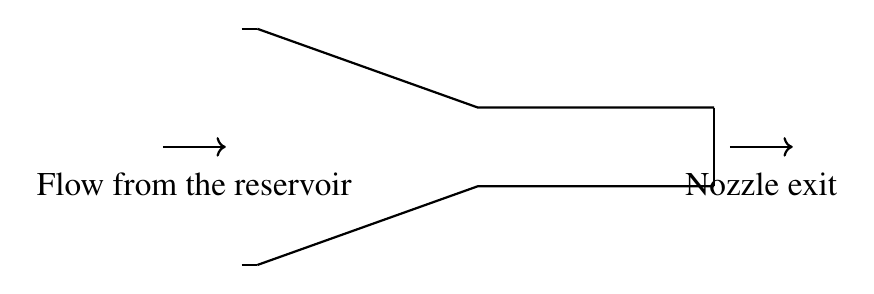
\begin{tikzpicture}
    % Draw the nozzle shape with short vertical lines at the opening
    \draw[thick] (-3,1.5) -- (-2.8,1.5);
    \draw[thick] (-3,-1.5) -- (-2.8,-1.5);
    \draw[thick] (-2.8,1.5) -- (0,0.5) -- (3,0.5);
    \draw[thick] (-2.8,-1.5) -- (0,-0.5) -- (3,-0.5);
    
    % Vertical line at the nozzle exit
    \draw[thick] (3,0.5) -- (3,-0.5);

    % Flow direction arrows
    \draw[->, thick] (-4,0) -- (-3.2,0);
    \draw[->, thick] (3.2,0) -- (4,0);

    % Labels for the flow and nozzle exit, placed below arrows
    \node[below] at (-3.6,-0.2) {\large Flow from the reservoir};
    \node[below] at (3.6,-0.2) {\large Nozzle exit};
\end{tikzpicture}


\begin{enumerate}
    \item $C=5\times 10^{-5}, \; \lambda=3\times 10^{-2}$
    \item $C=3\times 10^{-2}, \; \lambda=5\times 10^{-5}$
    \item $C=3\times 10^{-2}, \; \lambda=2\times 10^{4}$
    \item $C=2\times 10^{4}, \; \lambda=3\times 10^{-2}$
\end{enumerate}
\item A plane polarized electromagnetic wave in free space at time $t=0$ is given by $\overrightarrow{E}\brak{x, z}=10j\exp{\sbrak{i\brak{6x+8z}}}$. The magnetic field $\overrightarrow{B}\brak{x, z, t}$ is given by
\begin{enumerate}
    \item $\overrightarrow{B}\brak{x, z, t}=\frac{1}{c}\brak{6k-8\hat{i}}\exp{\sbrak{i\brak{6x+8z-10ct}}}$
    \item $\overrightarrow{B}\brak{x, z, t}=\frac{1}{c}\brak{6k+8\hat{i}}\exp{\sbrak{i\brak{6x+8z-10ct}}}$
    \item $\overrightarrow{B}\brak{x, z, t}=\frac{1}{c}\brak{6k-8\hat{i}}\exp{\sbrak{i\brak{6x+8z-ct}}}$
    \item $\overrightarrow{B}\brak{x, z, t}=\frac{1}{c}\brak{6k+8\hat{i}}\exp{\sbrak{i\brak{6x+8z+ct}}}$
\end{enumerate}
\item The eigenvalues of the matrix $\begin{bmatrix}
0 & 1 & 0 \\
1 & 0 & 1 \\
0 & 1 & 0 \\
\end{bmatrix}$ are
\begin{enumerate}
    \item $0, 1, 1$
    \item $0$, -$\sqrt{2}$, $\sqrt{2}$
    \item $\frac{1}{\sqrt{2}}$, $\frac{1}{\sqrt{2}}$, $0$
    \item $\sqrt{2}$, $\sqrt{2}$, $0$
\end{enumerate}
\item Match the typical spectroscopic regions specified in \textbf{Group I} with the corresponding type of transitions in \textbf{Group II.} \\
\begin{tabular}{ll}
    \textbf{Group I} & \textbf{Group II} \\
    \brak{P} Infra-red region          & \brak{i} electronic transitions involving valence electrons         \\
    \brak{Q} Ultraviolet-visible region         & \brak{ii} nuclear transitions        \\
    \brak{R} X-ray region        & \brak{iii} vibrational transitions of molecules    \\
    \brak{S} $\gamma$-ray region         & \brak{iv} transitions involving inner shell electrons        \\
\end{tabular}

\begin{enumerate}
    \item \brak{P,i}; \brak{Q,iii}; \brak{R, ii}; \brak{S, iv}
    \item \brak{P,ii}; \brak{Q,iv}; \brak{R, i}; \brak{S, iii}
    \item \brak{P,iii}; \brak{Q,i}; \brak{R, iv}; \brak{S, ii}
    \item \brak{P,iv}; \brak{Q,i}; \brak{R, ii}; \brak{S, iii}
\end{enumerate}
\item In the following circuit, for the output voltage to be $V_o=\brak{-V_1+\frac{V_2}{2}}$, the ratio $\frac{R_1}{R_2}$ is
% figure 2
	\begin{figure}[!ht]
\centering
\resizebox{3cm}{3cm}{%
\begin{circuitikz}
\tikzstyle{every node}=[font=\LARGE]
\draw [ line width=0.6pt](2.75,12) to[sinusoidal voltage source, sources/symbol/rotate=auto] (3.25,11.5);
\draw [ line width=0.6pt](3.25,11.75) to[european resistor] (9.5,11.75);
\draw [line width=0.6pt, ->, >=Stealth] (9.5,11.75) -- (9.5,11);
\draw [ line width=0.6pt](4,12.25) to[short] (4,11.25);
\draw [ line width=0.6pt](4,11.5) to[short] (4,11);
\draw [ line width=0.6pt](8.75,12.25) to[short] (8.75,11);
\draw [ line width=0.6pt](4,11.25) to[short] (4.5,11.25);
\draw [ line width=0.6pt](8.75,11.25) to[short] (8.25,11.25);
\draw [ line width=0.6pt](4.25,11.25) to[short] (5.25,11.25);
\draw [ line width=0.6pt](8.25,11.25) to[short] (7.25,11.25);
\draw [ line width=0.6pt](5,11.25) to[european resistor] (5,8.5);
\draw [ line width=0.6pt](7.5,11.25) to[european resistor] (7.5,8.5);
\draw [ line width=0.6pt](4.75,8.5) to[short] (8,8.5);
\draw [line width=0.6pt, ->, >=Stealth] (6.25,8.5) -- (6.25,7.75);
\node [font=\normalsize] at (6.75,8) {Bus 3};
\node [font=\normalsize] at (4,12.5) {Bus 1};
\node [font=\normalsize] at (8.75,12.5) {Bus 2};
\node [font=\normalsize] at (6.25,12.25) {j q};
\node [font=\normalsize] at (4.5,10) {j r};
\node [font=\normalsize] at (8.25,9.75) {j p};
\end{circuitikz}
}%

\label{fig:my_label}
\end{figure}

\begin{enumerate}
    \item $\frac{1}{2}$
    \item $1$
    \item $2$
    \item $3$
\end{enumerate}
\item The terms $\{\text{j}_1, \text{j}_2\}_J$ arising from $2\text{s}^13\text{d}^1$ electronic configuration in j-j coupling scheme are 
\begin{enumerate}
    \item $\{\frac{1}{2}, \frac{3}{2}\}_{2,1} \text{and} \{\frac{1}{2}, \frac{5}{2}\}_{3,2}$
    \item $\{\frac{1}{2}, \frac{1}{2}\}_{1,0} \text{and} \{\frac{1}{2}, \frac{3}{2}\}_{2,1}$
    \item $\{\frac{1}{2}, \frac{1}{2}\}_{1,0} \text{and} \{\frac{1}{2}, \frac{5}{2}\}_{3,2}$
    \item $\{\frac{3}{2}, \frac{1}{2}\}_{2,1} \text{and} \{\frac{1}{2}, \frac{5}{2}\}_{3,2}$
\end{enumerate}
\item In the following circuit, the voltage drop across the ideal diode in forward bias condition is $0.7V$.\\
%figure 3
	\begin{figure}[!ht]
\centering
\resizebox{3cm}{3cm}{%
\begin{circuitikz}
\tikzstyle{every node}=[font=\small]
\draw (4.25,12.25) to[battery1] (4.25,7.75);
\draw (4.25,12.25) to[short] (6.25,12.25);
\draw (4.25,7.75) to[short] (6.25,7.75);
\draw (6.25,12.25) to[R] (6.25,10.25);
\draw (6.25,10.25) to[R] (6.25,7.75);
\draw (6.25,10.25) to[short] (8.75,10.25);
\draw (6.25,7.75) to[short] (8.75,7.75);
\draw (8.75,7.75) to[R] (8.75,9.25);
\draw (8.75,10.25) to[D] (8.75,9);
\node [font=\small] at (4,10.25) {+};
\node [font=\small] at (4,9.75) {-};
\node [font=\small] at (4.75,10.5) {24 Volt};
\node [font=\small] at (6.75,11.25) {12 k$\Omega$};
\node [font=\small] at (6.75,9) {6 k$\Omega$};
\node [font=\small] at (8,8.5) {3.3 k$\Omega$};
\end{circuitikz}
}%

\label{fig:my_label}
\end{figure}

	The current passing through the diode is 

\begin{enumerate}
    \item $0.5$ mA
    \item $1.0$ mA
    \item $1.5$ mA
    \item $2.0$ mA
\end{enumerate}
\item Choose the CORRECT statement from the following.
\begin{enumerate}
    \item Neutron interacts through electromagnetic interaction
    \item Electron does not interact through weak interaction
    \item Neutrino interacts through weak and electromagnetic interaction
    \item Quark interacts through strong interaction but not through weak interaction
\end{enumerate}
\item A rod of proper length $l_o$ oriented parallel to the $x$-axis moves with speed $\frac{2c}{3}$ along the $x$-axis in the $S$-frame, where $c$ is the speed of the light in free space. The observer is also moving along the $x$-axis with speed $\frac{c}{2}$ with respect to the $S$-frame. The length of the rod as measured by the observer is
\begin{enumerate}
    \item $0.35l_o$
    \item $0.48l_o$
    \item $0.87l_o$
    \item $0.97l_o$
\end{enumerate}
\item A simple cubic crystal with lattice parameter $a_c$ undergoes transition into a tetragonal structure with lattice parameters $a_t=b_t=\sqrt{2}a_c$ and $c_t=2a_c$, below a certain temperature. The ratio of the interplanar spacings of $\brak{1 \; 0 \; 1}$ planes for the cubic and the tetragonal structure is
\begin{enumerate}
    \item $\sqrt{\frac{1}{6}}$
    \item $\frac{1}{6}$
    \item $\sqrt{\frac{3}{8}}$
    \item $\frac{3}{8}$
\end{enumerate}
\item Consider the following circuit in which the current gain $\beta_{dc}$ of the transistor is 100.
%figure 4
	\begin{figure}[H]
\centering
\resizebox{3cm}{3cm}{%
\begin{circuitikz}
\tikzstyle{every node}=[font=\small]
\draw [->, >=Stealth] (3.5,10.75) -- (3.5,13.75);
\draw [->, >=Stealth] (3.5,10.75) -- (10.75,10.75);
\draw [->, >=Stealth] (2.25,10.75) -- (3.25,10.75);
\draw [dashed] (4.5,13.25) -- (4.5,8.25);
\draw [dashed] (7.25,13.25) -- (7.25,8.25);
\draw [dashed] (10,13.25) -- (10,8.25);
\draw [dashed] (2,8.25) -- (10,8.25);
\draw [dashed] (2,13) -- (10,13);
\draw [short] (4.5,10.75) -- (7.25,11.75);
\draw [short] (7.25,11.75) -- (10,9.75);
\draw [short] (4.5,10.75) -- (10,9.75);
\node [font=\small] at (2.5,11) {$M>1$};
\node [font=\small] at (3.5,14) {$y$};
\node [font=\small] at (11,10.75) {$x$};
\node [font=\small] at (4.5,8) {$X_A$};
\node [font=\small] at (7.25,8) {$X_B$};
\node [font=\small] at (10,8) {$X_C$};
\node [font=\small] at (1.75,8.25) {$Y_{II}$};
\node [font=\small] at (1.75,13) {$Y_I$};
\node [font=\small] at (5.5,11) {$\alpha$};
\node [font=\small] at (6.5,10.5) {$\alpha$};
\node [font=\small] at (9,10) {$2\alpha$};
\end{circuitikz}
}%
\label{fig:my_label}
\end{figure}

	Which one of the following correctly represents the load line (collector current $I_C$ with respect to collector-emitter voltage $V_{CE}$) and $Q$-point of this circuit?
\begin{enumerate}
    \item
    %figure 5
	    \begin{figure}[!ht]
\centering
\resizebox{3cm}{3cm}{%
\begin{circuitikz}
\tikzstyle{every node}=[font=\small]
\draw [line width=0.6pt, short] (4,10.75) -- (8.25,10.75);
\draw [line width=0.6pt, short] (8.25,10.75) -- (9.75,12);
\draw [line width=0.6pt, short] (8.25,10.25) -- (9.75,11.5);
\draw [line width=0.6pt, short] (8.25,10.25) -- (9.75,9.25);
\draw [line width=0.6pt, short] (4,9.75) -- (8.25,9.75);
\draw [line width=0.6pt, ->, >=Stealth] (9.75,11.75) -- (10.25,12.25);
\draw [line width=0.6pt, ->, >=Stealth] (9.5,9) -- (10,8.5);
\draw [line width=0.6pt, ->, >=Stealth] (3.75,10.25) -- (5,10.25);
\node [font=\small] at (3.5,10.25) {$Q$};
\node [font=\small] at (10.5,12.5) {$Q_1$};
\node [font=\small] at (10.25,8.25) {$Q_2$};
\draw [line width=0.6pt, short] (8.25,9.75) -- (9.25,9);
\end{circuitikz}
}%

\end{figure}

    \item 
    %figure 6
	    \begin{figure}[H]
\centering
\resizebox{3cm}{3cm}{%
\begin{circuitikz}
\tikzstyle{every node}=[font=\large]
\draw [ line width=0.6pt ] (5.5,12.5) rectangle (7.5,6.25);
\draw [line width=0.6pt, dashed] (6.5,12.5) -- (6.5,6.25);
\draw [line width=0.6pt, dashed] (4.75,12.5) -- (8.5,12.5);
\draw [line width=0.6pt, dashed] (4.75,12.75) -- (8.5,12.75);
\draw [line width=0.6pt, dashed] (4.75,13) -- (8.5,13);
\draw [line width=0.6pt, dashed] (4.75,13.25) -- (8.5,13.25);
\draw [line width=0.6pt, dashed] (4.75,13.5) -- (8.5,13.5);
\draw [line width=0.6pt, ->, >=Stealth] (4.5,10.5) -- (4.5,8.75);
\draw [line width=0.6pt, <->, >=Stealth] (8.5,12.5) -- (8.5,6.25);
\node [font=\large] at (4,9.75) {$g$};
\node [font=\large] at (9.25,9.5) {L};
\end{circuitikz}
}%

\label{fig:my_label}
\end{figure}

    \item 
    %figure 7
	    \begin{figure}[H]
\centering
\resizebox{3cm}{3cm}{%
\begin{circuitikz}
\tikzstyle{every node}=[font=\small]
\draw [line width=1.4pt, short] (8,13) -- (8,7.25);
\draw [line width=0.6pt, short] (3,7.25) -- (10.5,7.25);
\draw [line width=0.6pt, short] (3,7.25) -- (3,13);
\draw [line width=0.6pt, short] (3,12.75) -- (8,12.75);
\draw [line width=0.6pt, short] (3,10.75) -- (8,10.75);
\draw [line width=0.6pt, <->, >=Stealth] (3.75,12.75) -- (3.75,10.75);
\draw [line width=0.6pt, <->, >=Stealth] (3.75,10.75) -- (3.75,7.25);
\draw [line width=0.6pt, ->, >=Stealth] (8.75,11.75) -- (8.75,10.75);
\node [font=\small] at (3.25,11.75) {$1\; m$};
\node [font=\small] at (3.25,9) {$2\;m$};
\node [font=\small] at (5.5,11.75) {$1000\; \frac{kg}{m^3}$};
\node [font=\small] at (5.5,9) {$2000 \;\frac{kg}{m^3}$};
\node [font=\small] at (6,6.5) {Not to scale};
\node [font=\small] at (9,11.25) {$g$};
\node [font=\small] at (9,13) {$P_a$};
\node [font=\small] at (5.25,13.25) {$P_a$};
\node [font=\Huge] at (8,7.5) {.};
\draw [line width=0.6pt, ->, >=Stealth] (8.25,7.5) -- (8.75,8);
\node [font=\small] at (9.25,8.25) {Hinge};
\end{circuitikz}
}%

\label{fig:my_label}
\end{figure}

    \item 
    %figure 8
	        \begin{figure}[H]
\raggedright
\resizebox{3cm}{3cm}{%
\begin{circuitikz}
\tikzstyle{every node}=[font=\small]
\draw [->, >=Stealth] (0.5,8) -- (0.5,12.5);
\draw [->, >=Stealth] (0.5,8) -- (6.5,8);
\draw [->, >=Stealth] (7,8) -- (13.25,8);
\draw [->, >=Stealth] (7,8) -- (7,12.5);
\draw [dashed] (1,12) -- (1,8.5);
\draw [dashed] (3,12) -- (3,8.75);
\draw [dashed] (5,12) -- (5,8.5);
\draw [short] (0.5,9.5) -- (1,9.5);
\draw [short] (1,9.5) -- (1,11.5);
\draw [short] (1,11.5) -- (3.5,11.5);
\draw [short] (3.5,11.5) -- (4.25,9.25);
\draw [short] (4.25,9.25) -- (5,9.25);
\draw [dashed] (7.5,12.25) -- (7.5,8.75);
\draw [dashed] (9.5,12.25) -- (9.5,8.75);
\draw [dashed] (12,12.25) -- (12,9);
\node [font=\small] at (8.5,12) {$Y_{II}$};
\node [font=\small] at (7.5,8.5) {$X_A$};
\node [font=\small] at (9.5,8.5) {$X_B$};
\node [font=\small] at (12,8.75) {$X_C$};
\node [font=\small] at (1,8.25) {$X_A$};
\node [font=\small] at (3,8.5) {$X_B$};
\node [font=\small] at (5,8.5) {$X_C$};
\node [font=\small] at (6.5,11.25) {P};
\node [font=\small] at (0.25,11.5) {P};
\node [font=\small] at (4,7.75) {$x$};
\node [font=\small] at (10.5,7.75) {$x$};
\node [font=\small] at (1.75,11.75) {$Y_I$};
\draw [short] (7,9.5) -- (8,9.5);
\draw [short] (8,9.5) -- (8,11.75);
\draw [short] (8,11.75) -- (12,11.75);
\end{circuitikz}
}%

\end{figure}

   \end{enumerate}
\item Consider a system whose three energy levels are given by 0, $\epsilon$ and $2\epsilon$. The energy level $\epsilon$ is two-fold degenerate and the other two are non-degenerate. The partition function of the system with $\beta=\frac{1}{k_BT}$
\begin{enumerate}
    \item $1+2e^{-\beta \epsilon}$
    \item $2e^{-\beta \epsilon}+e^{-2\beta \epsilon}$
    \item $\brak{1+e^{-\beta \epsilon}}^2$
    \item $1+e^{-\beta \epsilon}+e^{-2\beta \epsilon}$
\end{enumerate}
\item Two infinitely extended homogeneous isotropic dielectric media (medium-1 and medium-2 with dielectric constants $\frac{\epsilon_1}{\epsilon_2}=2$ and $\frac{\epsilon_2}{\epsilon_0}=5$, respectively) meet at the $z=0$ plane as shown in the figure . A uniform electric field exists everywhere. For $z \geq 0$, the electric field is given by $\overrightarrow{E_1}=2\hat{1}-3j+5k$. The interface separating the two media is charge free.\\ The electric displacement vector in the medium-2 is given by 
	\begin{figure}[!ht]
\centering
\resizebox{3cm}{3cm}{%
\begin{circuitikz}
\tikzstyle{every node}=[font=\small]
\draw [->, >=Stealth] (7.5,8.25) -- (7.5,12.5);
\draw [dashed] (5.25,10.25) -- (10,10.25);
\node [font=\small] at (5.5,9.5) {medium2};
\node [font=\small] at (5.25,11.25) {medium-1};
\node [font=\small] at (9.25,10) {z=0};
\end{circuitikz}
}%

\label{fig:my_label}
\end{figure}

	\begin{enumerate}
    \item $\overrightarrow{D_2}=\epsilon_0\sbrak{10\hat{i}+15j+10k}$
    \item $\overrightarrow{D_2}=\epsilon_0\sbrak{10\hat{i}-15j+10k}$
    \item $\overrightarrow{D_2}=\epsilon_0\sbrak{4\hat{i}-6j+10k}$
    \item $\overrightarrow{D_2}=\epsilon_0\sbrak{4\hat{i}+6j+10k}$
\end{enumerate}

\end{enumerate}
\end{document}
